%!TEX ROOT=../diploma-thesis.tex

\chapter{Anal\'yza}\label{ch:analyza}

Tato kapitola analyzuje problematiku byznysov\'ych pravidel v informačn\'{\i}ch systémech.
Dále detailně popisuje architekturu orientovanou na služby, včetně jej\'{\i}ho historického
v\'yvoje a modern\'{\i}ho trendu v podobě microservices. Na základě toho kapitola popisuje nedostatky
současn\'ych př\'{\i}stupů při řešen\'{\i} průřezov\'ych problémů v těchto architekturách, s důrazem na byznysová pravidla.
V závěru kapitoly jsou identifikovány požadavky, které by měl splňovat framework,
jež bude v\'ystupem této diplomové práce.

\section{Byznysová pravidla}\label{sec:business-rules}

Informačn\'{\i} systémy (\gls{IS}) maj\'{\i} za úkol ulehčit, automatizovat či poskytovat podporu pro
byznysové procesy společnost\'{\i}, které je využ\'{\i}vaj\'{\i}. Tyto procesy jsou tedy stěžejn\'{\i}m
prvkem \gls{IS}. Systém má také za úkol uchovávat a spravovat data společnosti
a měl by zaručit, že nedojde k jejich poškozen\'{\i} či narušen\'{\i} jejich integrity.
Byznysové procesy, potažmo byznysové operace, proto musej\'{\i}
podléhat jasně definovan\'ym byznysov\'ym pravidlům, která zajišťuj\'{\i} konzistenci dat informačn\'{\i}ho
systému a také zabraňuj\'{\i} nepovolen\'ym operac\'{\i}m~\cite{cemus2015automated}.

Byznysová pravidla děl\'{\i}me do tř\'{\i} skupin~\cite{cemus2014aspect}:
\begin{description}
    \item [Bezkontextová pravidla] jsou validačn\'{\i} pravidla, která musej\'{\i} b\'yt obecně platná
    v každé operaci, jinak by mohlo doj\'{\i}t k porušen\'{\i} integrity dat systému. Př\'{\i}kladem může
    b\'yt pravidlo \uv{\textit{Adresa uživatele je platnou e-mailovou adresou}}.
    \item [Kontextová pravidla] jsou pravidla, která musej\'{\i} b\'yt zohledněna v daném kontextu
    byznysové operace, např\'{\i}klad \uv{\textit{Při přidán\'{\i} produktu do koš\'{\i}ku nesm\'{\i} součet položek
    v koš\'{\i}ku přesahovat částku milion korun}}
    \item [Průřezová pravidla] jsou parametrizována stavem systému nebo uživatelského účtu a maj\'{\i}
    dopad na velkou část byznysov\'ych operac\'{\i}. Uvažme pravidlo \uv{\textit{V systému nesm\'{\i} prob\'{\i}hat
    žádné změny po dobu účetn\'{\i} uzávěrky}}.
\end{description}

Dále také rozlišujeme dva typy byznysov\'ych pravidel, a těmi jsou \textit{preconditions}
a \textit{post-conditions}~\cite{cemus2015automated}.

\subsection{Precondition}

Aby mohla b\'yt byznysová operace vykonána, musej\'{\i}
b\'yt splněny předem definované podm\'{\i}nky, neboli předpoklady,
které naz\'yváme \textit{preconditions}. Pokud alespoň jedna z podm\'{\i}nek
nen\'{\i} splněna, byznysová operace nemůže proběhnout.

Pro lepš\'{\i} ilustraci uveďme př\'{\i}klad: aby mohla b\'yt provedena
registrace uživatele s danou emailovou adresu, mus\'{\i} b\'yt splněna
podm\'{\i}nka, že uživatel vyplnil svoj\'{\i} emailovou adresu, a zároveň
dosud v systému neexistuje žádn\'y uživatel se stejnou emailovou adresou.

\subsection{Post-condition}

Na byznysovou operaci mohou b\'yt kladeny požadavky, které
musej\'{\i} b\'yt splněny po jej\'{\i}m úspěšném vykonán\'{\i}. Př\'{\i}kladem
může b\'yt anonymizace uživatelů při vytvářen\'{\i} statistického
reportu e-commerce společnosti – po vygenerován\'{\i} reportu
post-condition zajist\'{\i}, že z něj budou smazány veškeré citlivé údaje.
Dalš\'{\i}m př\'{\i}padem může b\'yt filtrován\'{\i} v\'ystupu byznysové operace.
Např\'{\i}klad při v\'ypisu objednávek pro zákazn\'{\i}ka se chceme ujistit, že
všechny vypsané objednávky patř\'{\i} danému zákazn\'{\i}kovi.

\subsection{Reprezentace byznysového pravidla}

Existuje několik možnost\'{\i}, jak zachytit a reprezentovat byznysová pravidla~\cite{cemus2015automated}.
Nejběžnějš\'{\i} a nejpouž\'{\i}vanějš\'{\i} metodou je jejich zachycen\'{\i} v programovac\'{\i}m
jazyce. Tato metoda je snadná, protože programátor může použ\'{\i}t stejn\'y jazyk
pro popis pravidel stejně jako pro popis celého systému. Bohužel, tato metoda
nám nedává př\'{\i}liš možnost\'{\i} jak provést inspekci a extrakci pravidel.
Dalš\'{\i}, pokročilejš\'{\i} metodou, je zápis pravidel pomoc\'{\i} meta-instrukc\'{\i}, např\'{\i}klad anotac\'{\i},
nebo tzv.\textit{Expression Language} (\gls{EL}). Tato metoda poskytuje dobrou možnost inspekce,
ale zpravidla nen\'{\i} typově bezpečná a může snáze způsobovat chyby v programu.
Posledn\'{\i}, nejpokročilejš\'{\i} metodou, je zápis pomoc\'{\i} doménově specifick\'ych jazyků.
Ty jsou snadno srozumitelné nejen pro programátory, ale i pro doménové experty.
Nevyžaduj\'{\i} inspekci a mohou b\'yt typově bezpečné. Mezi jejich nev\'yhody ale patř\'{\i} vysoká
počátečn\'{\i} investice v podobě návrhu takového jazyka a nutnost jeho kompilace nebo
interpretace.

\subsection{Byznysov\'y kontext}

Informačn\'{\i} systém zpravidla implementuje v\'{\i}ce byznysov\'ych procesů, které se vážou
na jeden či v\'{\i}ce uživatelsk\'ych scénářů. Uživatelsk\'y scénář se pak děl\'{\i} na jednotlivé
kroky, např\'{\i}klad zaslán\'{\i} potvrzovac\'{\i}ho e-mailu k objednávce, či uložen\'{\i} objednávky
do databáze. Tyto kroky naz\'yváme \textit{byznysové operace} – tedy operace, které maj\'{\i}
byznysovou hodnotu. Ke každé byznysové operaci př\'{\i}sluš\'{\i} množina byznysov\'ych pravidel,
konkrétně preconditions a post-conditions.

Při běhu informačn\'{\i}ho systému je v paměti držen tzv. \textit{exekučn\'{\i} kontext} (z anglického \textit{execution context}),
kter\'y se skládá z několika d\'{\i}lč\'{\i}ch kontextů~\cite{cemus2017separation}. Prvn\'{\i}m
je \textit{aplikačn\'{\i} kontext} (z anglického \textit{application context}), ve kterém je uložen stav globálnc\'{\i}h proměnn\'ych systému,
jako např. nastaven\'{\i} produkčn\'{\i}ho režimu, nebo př\'{\i}znak o tom, zda právě prob\'{\i}há obchodn\'{\i}
uzávěrka. Dalš\'{\i}m je \textit{uživatelsk\'y kontext}, kter\'y obsahuje informace o aktuálně
přihlášeném uživateli. \textit{Kontext požadavku} (z anglického \textit{Request context}) obsahuje
informace o aktuáln\'{\i}m požadavku, jako IP adresa uživatele či jeho geolokace,
a vztahuje se zejména k webov\'ym službám. Posledn\'{\i}m je \textit{byznysov\'y kontext}. Ten
chápeme jako množinu preconditions a post-conditions s byznysovou hodnotou, která se
váže na konkrétn\'{\i} byzynsovou operaci~\cite{cemus2015automated}.
Abychom mohli efektivně definovat co nejširš\'{\i} škálu byzynsov\'ych pravidel,
musej\'{\i} při jejich vyhodnocován\'{\i} b\'yt dostupné proměnné exekučn\'{\i}ho kontextu,

\section{Architektura orientovaná na služby}\label{sec:soa}

\goal{Úvod do SOA, proč je potřeba}
V posledn\'{\i}ch dekádách můžeme sledovat trend nárůstu komplexity
modern\'{\i}ch informačn\'{\i}ch systémů, kter\'y je způsoben stále náročnějš\'{\i}mi
požadavky na jejich funkcionalitu, v\'ykon a spolehlivost. To nut\'{\i}
v\'yvojáře těchto systémů přizpůsobovat architekturu systému tak,
aby uměla splnit všechny očekávané funkčn\'{\i} i nefunkčn\'{\i} požadavky,
zejména pak škálovatelnost systému a jeho schopnost zvládat vysok\'y
objem dat a uživatelů. \textit{Architektura orientovaná na služby} (\gls{SOA}) je
důsledkem této evoluce. Na rozd\'{\i}l od dř\'{\i}vě běžné a dnes
stále použ\'{\i}vané \textit{monolitické architektury},
\gls{SOA} podle známého pravidla \uv{rozděl a panuj}
děl\'{\i} systém na samostatné celky, zvané \textit{služby}, které jsou
zodpovědné za d\'{\i}lč\'{\i} část požadované funkcionality.

\goal{Proč tu vlastně p\'{\i}šu o nějaké historii}
Historicky byl term\'{\i}n \gls{SOA} vykládán různ\'ymi způsoby a v\'yvojáři si
pod n\'{\i}m představovali několik rozd\'{\i}ln\'ych, nekompatibiln\'{\i}ch
konceptů~\cite{fowler2005serviceorientedambiguity}.
Zejména pak absence kvalitn\'{\i}ch definic toho, co vlastně
služba je, vedla k vzájemnému nedorozuměn\'{\i}, zmaten\'{\i} a v posledn\'{\i}
době i ke snahám o opuštěn\'{\i} tohoto konceptu~\cite{cerny2017disambiguation}.
Abychom lépe prozuměli tomu, co vlastně \gls{SOA} je, pop\'{\i}šeme si jej\'{\i} historick\'y
v\'yvoj a shrneme v\'yhody a nev\'yhody jednotliv\'ych př\'{\i}stupů.

\subsection{Common Object Request Broker Architecture}\label{sec:corba}

Prvn\'{\i}m historick\'ym předchůdcem architektury orientované na služby
byla tzv. \textit{Common Object Request Broker Architecture}
(\gls{CORBA})~\cite{siegel2000corba}, která vzikala v osmdesát\'ych a devadesát\'ych letech
dvacátého stolet\'{\i}. Ta umožňuje komunikaci mezi aplikacemi implementovan\'ymi v
různ\'ych technologi\'{\i}ch a běž\'{\i}c\'{\i}mi na vlastn\'{\i}ch stroj\'{\i}ch s rozd\'{\i}ln\'ymi
operačn\'{\i}mi systémy. Základn\'{\i}m stavebn\'{\i}m kamenem této architektury
je \textit{Object Request Broker} (\gls{ORB}), kter\'y emuluje objekty,
na kter\'ych může klient volat jejich metody. Při zavolán\'{\i} metody
na objektu, kter\'y se fyzicky nacház\'{\i} v aplikaci na vzdáleném stroji,
zprostředkovává \gls{ORB} veškerou komunikaci a svému uživateli poskytuje
jeho kompletn\'{\i} rozhran\'{\i}. Uživatel tedy de facto nerozezná, kdy volá
metodu na objektu, kter\'y je lokálně dostupn\'y,
a kdy volá metodu, kterou obsouž\'{\i} vzdálená služba. To je ale zároveň
hlavn\'{\i} nev\'yhodou této architektury, protože komunikace se vzdálen\'ym
objektem s sebou nese celou řadu problémů, např\'{\i}klad mnohem vyšš\'{\i} latenci
při komunikaci nebo v\'yjimečné stavy, které je potřeba ošetřit. Ve chv\'{\i}li,
kdy klient nen\'{\i} schopen rozeznat mezi metodou volanou lokálně či vzdáleně,
se těžko přizpůsobuje těmto okolnostem, což vnáš\'{\i} do kódu zbytečnou
komplexitu a zhoršuje jeho kvalitu kvůli obt\'{\i}žnějš\'{\i} optimalizaci.

\subsection{Web Services}

Nedostatky architektury \gls{CORBA} vedly k volbě jednodušš\'{\i}ho
formátu pro popis komunikace služeb, spolehlivějš\'{\i}ho a méně
komplikovaného kanálu pro komunikaci a celkové redukci
objemu komunikovan\'ych dat. Preferovanou cestou komunikace
se na přelomu tis\'{\i}cilet\'{\i} stal protokol \gls{HTTP}, zat\'{\i}mco preferovan\'ym formátem
pro serializaci přenášen\'ych dat se stal jazyk \gls{XML}.
Postupně se upustilo od volán\'{\i} metod na vzdálen\'ych objektech a přijal
se koncept explicitn\'{\i}ho pos\'{\i}lán\'{\i} zpráv mezi službami.
Pro popis schématu zpráv vznikl formát \textit{Simple Object Access
Protocol} (\gls{SOAP})~\cite{box2000simple}, kter\'y v kombinaci s
\textit{Web Service Description Language} (\gls{WSDL})~\cite{christensen2001web}
umožňuje kompletn\'{\i} definici rozhran\'{\i} pro komunikaci mezi službami.
V průběhu dalš\'{\i}ch let vznikla také velmi populárn\'{\i} architektura
\textit{Representational State Transfer} (\gls{REST})~\cite{fielding2000rest},
která pro popis webov\'ych služeb využ\'{\i}vá čistě protokol \gls{HTTP} a jeho slovesa.
To službám přináš\'{\i} společn\'y slovn\'{\i}k a umožňuje snažš\'{\i} dokumentaci
a rychlejš\'{\i} orientaci v\'yvojářů, kteř\'{\i} takovou službu implementuj\'{\i} či konzumuj\'{\i}.
Kvůli těžkopádnosti \gls{XML} se pro služby implementuj\'{\i}c\'{\i} \gls{REST} architekturu stal
preferovan\'ym formátem přenosu \textit{JavaScript Object Notation} (\gls{JSON}).
Nejnovějš\'{\i}m formátem pro popis služeb, čerpaj\'{\i}c\'{\i} z nedostatků architektury \gls{REST}, je
\textit{GraphQL}, se kter\'ym v roce 2015 přišla společnost Google.

\subsection{Message Queue}

\begin{figure}
    \centering
    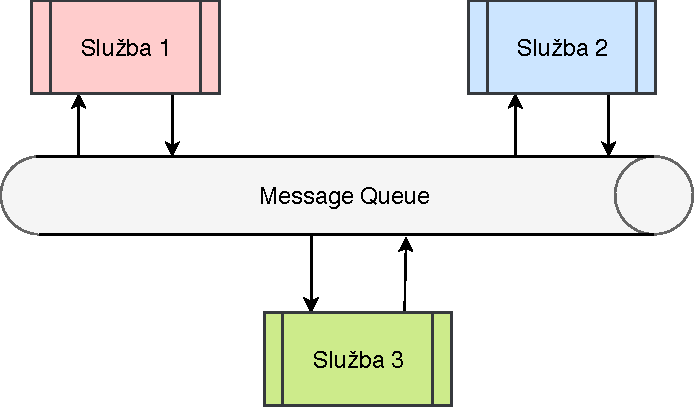
\includegraphics[keepaspectratio=true, width=0.5\linewidth]{figures/message-queue.pdf}
    \caption{Komunikace služeb pomoc\'{\i} Message Queue}
    \label{fig:message-queue}
\end{figure}

Dalš\'{\i}m z konceptů, kter\'y v rámci \gls{SOA} vznikl, je tzv. \textit{Message Queue} (\gls{MQ}).
Základn\'{\i} myšlenkou \gls{MQ}, znázorněnou na obrázku~\ref{fig:message-queue},
je asynchronn\'{\i} komunikace služeb pomoc\'{\i} zpráv nezávisl\'ych
na platformě. Komunikaci zprostředkovává fronta, která přij\'{\i}má a rozes\'{\i}lá
zprávy mezi službami. To přináš\'{\i} vyšš\'{\i} škálovatelnost a menš\'{\i} provázanost
mezi službami. Všechny služby ale mus\'{\i} použ\'{\i}vat jednotn\'y formát zpráv.

\gls{MQ} přináš\'{\i} dva způsoby, kter\'ymi mohou služby komunikovat. Prvn\'{\i}m je
\textit{Request/Reply}, připom\'{\i}naj\'{\i}c\'{\i} konverzaci dvou lid\'{\i}. Jedna
služba zašle zprávu obsahuj\'{\i}c\'{\i} identifikátor konverzace. Druhá služba
na obdrženou zprávu zašle odpověď a pomoc\'{\i} identifikátoru označ\'{\i},
ke které otázce odpověď patř\'{\i}. Druh\'ym způsobem je \textit{publish-subscribe},
kdy existuje v\'{\i}ce front s různ\'ymi tématy (\textit{topics}) a služby mohou
do těchto front přisp\'{\i}vat relevantn\'{\i}mi zprávami nebo je konzumovat jako odběratelé.

\subsection{Enterprise Service Bus}

Ačkoliv zm\'{\i}něné modely usnadňuj\'{\i} komunikaci služeb a zvyšuj\'{\i} jejich
spolehlivost, integrace služeb může b\'yt obt\'{\i}žná, pokud služby použ\'{\i}vaj\'{\i} navzájem různé
komunikačn\'{\i} protokoly a formáty. Již v devadesát\'ych letech minulého stolet\'{\i}
byl představen koncept \textit{Enterprise Service
Bus} (\gls{ESB})~\cite{chappell2004enterprise},
znázorněn\'y na obrázku~\ref{fig:enterprise-service-bus},
kter\'y má za úkol propojit heterogenn\'{\i} služby a zajistit mezi nimi
komunikačn\'{\i} kanály. T\'{\i}m na sebe \gls{ESB} přeb\'{\i}rá zodpovědnost za překlad
jednotliv\'ych zpráv a centralizuje veškerou komunikaci v systému.

\gls{ESB} se zároveň stav\'{\i} do role experta na lokalizaci jednotliv\'ych služeb.
Službě tak pro komunikaci s okoln\'{\i}m světem stač\'{\i} znát adresu \gls{ESB}, kterému
zašle zprávu, a ten ji sám doruč\'{\i} na m\'{\i}sto určen\'{\i}. Tento model ale
znamená, že \gls{ESB} je velmi komplexn\'{\i} komponentou. V\'ypadek \gls{ESB} nav\'{\i}c
v způsob\'{\i} zastaven\'{\i} funkce celého systému a \gls{ESB} se tak stává
tzv. \textit{single point of failure}, což v praxi snižuje škálovatelnost systému.
V př\'{\i}padě vlastn\'{\i}ho n\'{\i}zkého v\'ykonu se \gls{ESB} může snadno stát úzk\'ym hrdlem.
Tyto problémy mohou b\'yt částečně vyřešeny tzv. \textit{federovan\'ym designem},
kdy je systém rozdělen na byznysově př\'{\i}buzné části, z nichž každá má
svůj \gls{ESB}.

\begin{figure}
    \centering
    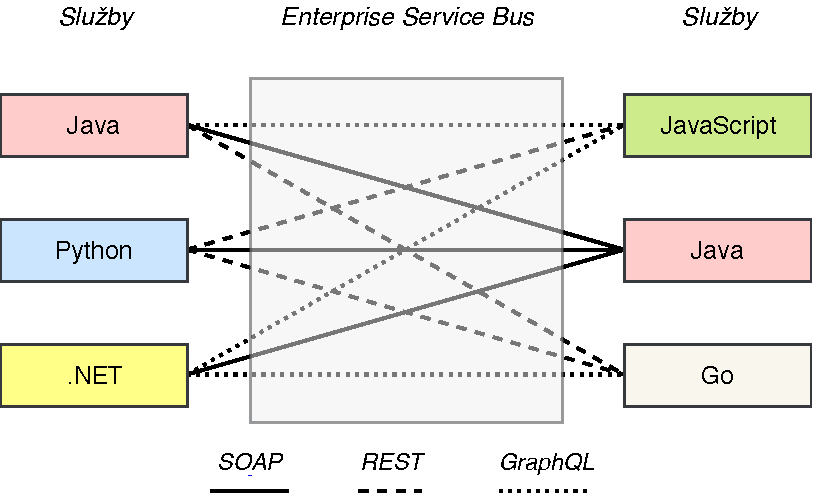
\includegraphics[keepaspectratio=true, width=0.7\linewidth]{figures/enterprise-service-bus.pdf}
    \caption{Komunikace služeb skrz Enterprise Service Bus}
    \label{fig:enterprise-service-bus}
\end{figure}

\subsection{Microservices}\label{sec:microservices}

\goal{Microservices a budoucnost SOA}
Nov\'ym trendem posledn\'{\i}ch let je architektura zvaná \textit{Microservices}.
Přináš\'{\i} několik zajmav\'ych konceptů, které specializuj\'{\i} a konkretizuj\'{\i}
principy \gls{SOA}. Microservices se tedy daj\'{\i} chápat jako podmnožina
\gls{SOA}, ačkoliv existují i názory, že jde o odlišné architektury~\cite{richards2015microservices}.
Základn\'{\i} myšlenkou je v\'yvoj informačn\'{\i}ho systému jako množiny
mal\'ych oddělen\'ych služeb, které jsou spouštěny v samostatn\'ych procesech
a komunikuj\'{\i} spolu pomoc\'{\i} jednoduch\'ych protokolů~\cite{lewis2014microservices}.

\goal{Stavba služeb kolem byznysov\'ych schopnost\'{\i}}
Důležitou myšlenkou microservices je organizace služeb kolem
byznysov\'ych schopnost\'{\i} systému. Nam\'{\i}sto horizontáln\'{\i}ho dělen\'{\i} systému
podle jeho vrstev\footnote{
Zde předpokládáme klasickou tř\'{\i}vrstvou architekturu~\cite{fowler2002patterns},
rozděluj\'{\i}c\'{\i} systém na \textit{datovou vrstvu}, \textit{aplikačn\'{\i} vrstvu}
a \textit{prezentačn\'{\i} vrstvu}. Tyto vrstvy maj\'{\i} oddělené zodpovědnosti a komunikuj\'{\i}
spolu pomoc\'{\i} jasně definovan\'ych společn\'ych rozhran\'{\i}.
} navrhuje rozdělit systém vertikálně podle jeho byznysov\'ych schopnost\'{\i}.
Na obrázku~\ref{fig:monolith-vs-microservices} je toto rozdělen\'{\i} demonstrováno.
Př\'{\i}kladem může b\'yt dělen\'{\i} e-commerce systému na jednu službu obsahuj\'{\i}c\'{\i} byznysovou
logiku pro registraci a správu uživatelů, druhou službu obsahuj\'{\i}c\'{\i} byznysovou logiku
pro práci s produkty a třet\'{\i} službu obsahuj\'{\i}c\'{\i} byznysovou logiku pro práci
s objednávkami.

\begin{figure}
    \centering
    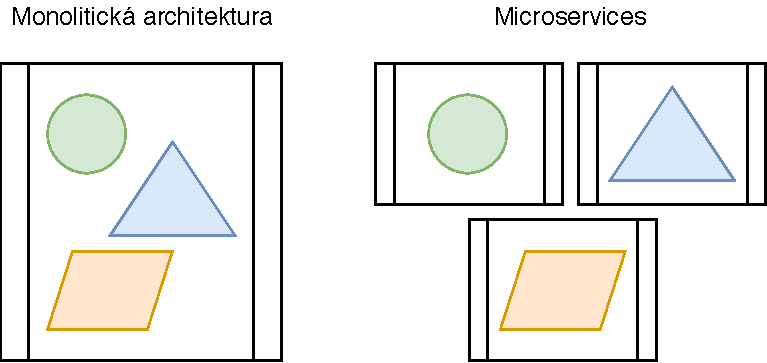
\includegraphics[keepaspectratio=true, width=0.5\linewidth]{figures/monolith-vs-microservices.pdf}
    \caption{Porovnán\'{\i} struktury monolitické architektury a microservices~\cite{lewis2014microservices}}
    \label{fig:monolith-vs-microservices}
\end{figure}

\goal{Myšlenka nahraditelnosti komponenty}
Koncept microservices přem\'yšl\'{\i} o službě jako o samostatné komponentě,
kterou lze individuálně vyměnit či vylepšit, bez nutnosti zásahu do
ostatn\'{\i}ch služeb~\cite{lewis2014microservices}. Monolitická architektura
vyžaduje i při malé změně jedné části cel\'y systém znovu zkompilovat, sestavit
a nasadit. Malé služby slouž\'{\i}c\'{\i} ideálně jedinému byznysovému účelu lze naopak
při změně byznysov\'ych požadavků snadno nahradit samostatně bez zásahu do zbytku
systému. T\'{\i}m se usnadňuje cyklus nasazen\'{\i} a spuštěn\'{\i} nové verze služby.

\goal{Myšlenka smart endpoints, dumb pipes}
Microservices také přinášej\'{\i} koncept \uv{smart endpoint, dumb pipes},
kter\'y opoušt\'{\i} koncept \gls{ESB} ve prospěch přesunut\'{\i} veškeré byznys logiky
na stranu služeb. T\'{\i}m se zvyšuje zapouzdřenost služeb a snižuje se
jejich vzájemné provázán\'{\i}. Nutno podotknout, že microservices často
využ\'{\i}vaj\'{\i} ke své funkci Message Queues.

\paragraph{Škálovatelnost}
Dalš\'{\i} nespornou v\'yhodou microservices je vysoká škálovatelnost systému. Pokud je na
některou ze služeb kladen vyšš\'{\i} nárok na v\'ykon než na ostatn\'{\i}, maj\'{\i}
v\'yvojáři možnost konkrétn\'{\i} službu horizontálně škálovat aniž by
museli škálovat kompletně cel\'y systém, na rozd\'{\i}l od monolitické architektury.
Srovnán\'{\i} př\'{\i}stupů je znázorněno na obrázku~\ref{fig:microservices-deployment}.
D\'{\i}ky této vlastnosti je možné sn\'{\i}žit nároky na systémové zdroje při zachován\'{\i}
stejného v\'ykonu.

\paragraph{Využit\'{\i} rozlišn\'ych technologi\'{\i}}
Monolitické aplikace jsou často implementovány v jednom programovac\'{\i}m jazyce
a využ\'{\i}vaj\'{\i} omezenou množinu technologi\'{\i}. Ne pro každ\'y úkol je ale vhodn\'y
jeden programovac\'{\i} jazyk a s rostouc\'{\i} velikost\'{\i} informačn\'{\i}ho systému často roste
i rozmanitost jeho funkcionality. Rozdělen\'{\i}m systému na v\'{\i}ce služeb, které
komunikuj\'{\i} protokolem nezávisl\'ym na platformě, je v\'yvojářům umožněno využ\'{\i}t
širš\'{\i} spektrum technologi\'{\i} a implementovat požadovanou funkcionalitu
efektivněji.

\begin{figure}
    \centering
    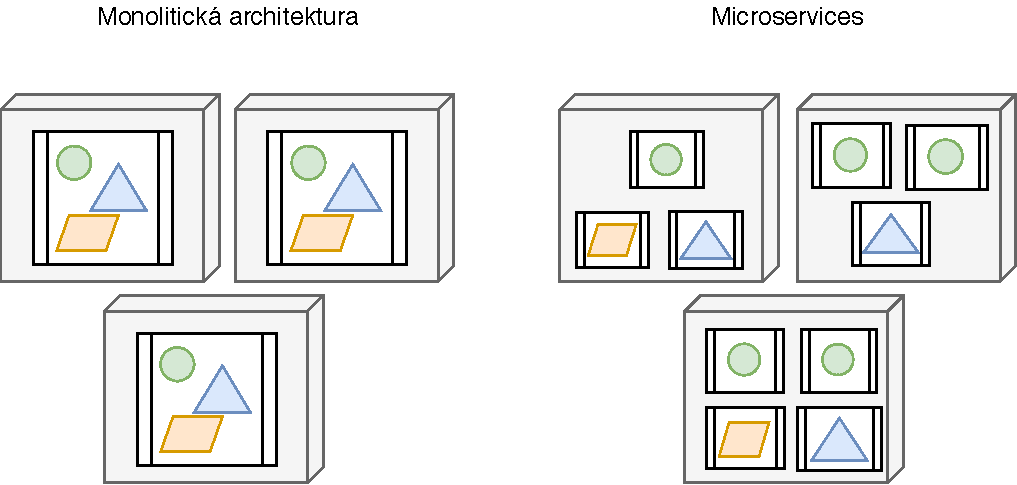
\includegraphics[keepaspectratio=true, width=0.8\linewidth]{figures/microservices-deployment.pdf}
    \caption{Porovnán\'{\i} nasazen\'{\i} monolitické architektury a microservices~\cite{lewis2014microservices}}
    \label{fig:microservices-deployment}
\end{figure}

\paragraph{Decentralizace úložiště}
Dalš\'{\i}m z principů, které microservices přináš\'{\i}, je oddělen\'{\i} a decentralizace
databázového úložiště. Každá služba, či cluster instanc\'{\i} jedné služby, zapisuj\'{\i}
a čtou data ze své oddělené databáze. Pokud potřebujou nač\'{\i}st data jiné služby,
musej\'{\i} k tomu využ\'{\i}t jej\'{\i} \gls{API}. T\'{\i}m se ještě v\'yrazněji odděluje zodpovědnost služeb.
Typickou praktikou v rámci \gls{SOA} je naopak sd\'{\i}len\'{\i} jedné databáze mezi v\'{\i}ce službami,
což je často dáno komerčn\'{\i}m modelem extern\'{\i}ho dodatavele databáze. Jediná databáze
má nav\'{\i}c obrovskou v\'yhodu v transakčn\'{\i}m zpracován\'{\i}, které je centralizované.
V př\'{\i}padě microservices je nutno transakce řešit distribuovaně, což je velmi náročn\'y
úkol a společnosti často vol\'{\i} koncept tzv. \textit{eventual consistency}, kdy je
preferována občasná nekonzistence v datech, která je následně manuálně opravena.
Tento př\'{\i}stup je opodstatněn t\'{\i}m, že občasná manuáln\'{\i} oprava může b\'yt
často levnějš\'{\i} než investice do kvalitn\'{\i}ho řešen\'{\i} distribuovan\'ych transakc\'{\i} –
zejména pokud by jeho řešen\'{\i} znamenalo zpožděn\'{\i} v\'yvoje produktu a způsobilo
by ztrátu obchodn\'{\i} př\'{\i}ležitosti~\cite{lewis2014microservices}.

\subsection{Orchestrace a choreografie služeb}

Jak již bylo zm\'{\i}něno, aby informačn\'{\i} systém skládaj\'{\i}c\'{\i} se ze služeb mohl vykonávat
své funkce, musej\'{\i} spolu služby komunikovat. Aby tato komunikace opravdu vedla
ke správné funkci systému, mus\'{\i} podléhat jasně danému řádu.

\paragraph{Orchestrace služeb}
Pro vykonán\'{\i} byznysové operace je v rámci \gls{SOA} často potřeba součinnost v\'{\i}ce služeb
najednou. \textit{Orchestrace služeb} má za úkol zajistit, že komunikace mezi službami
proběhne úspěšně a ve správném časovém sledu~\cite{orchestration},
pomoc\'{\i} centráln\'{\i} komponenty – tzv. \textit{dirigenta}.
Abychom si mohli tento koncept lépe představit, uvažme následuj\'{\i}c\'{\i} př\'{\i}klad. Uživatel
pomoc\'{\i} \gls{UI} vytvoř\'{\i} a odešle objednávku. V tuto chv\'{\i}li
je spuštěn byznysov\'y proces, kter\'y mus\'{\i} zajistit, že objednávka bude založena v databázi,
budou o n\'{\i} informováni skladn\'{\i}ci, bude zažádáno o vytvořen\'{\i} faktury a nakonec bude odeslán
potvrzovac\'{\i} e-mail zákazn\'{\i}kovi. Po úspěšném dokončen\'{\i} operace je nav\'{\i}c potřeba uživateli
zobrazit v \gls{UI} informaci, že vše proběhlo v pořádku. V př\'{\i}padě orchestrace služba
poskytuj\'{\i}c\'{\i} \gls{UI} požádá dirigenta o vytvořen\'{\i} objednávky a ten se již postará o
komunikaci tohoto požadavku všem službám zapojen\'ym do procesu.
Typicky je jako dirigent využ\'{\i}ván \gls{ESB}, kter\'y je pro tuto roli vhodn\'y,
protože má informace o lokaci jednotliv\'ych služeb a zprostředkovává mezi nimi
komunikačn\'{\i} kanály.

\paragraph{Choreografie služeb}
Př\'{\i}m\'ym opakem orchestrace je tzv. \textit{choreografie služeb} a znamená
vykonáván\'{\i} byznysov\'ych operac\'{\i} autonomně a asynchronně, bez centráln\'{\i}
autority. V př\'{\i}padě microservices je preferován tento př\'{\i}stup~\cite{dragoni2017microservices},
protože orchestrace vede k vyšš\'{\i}mu provázán\'{\i} služeb a nerovnoměrnému rozložen\'{\i}
zodpovědnost\'{\i} v systémů. Porovnán\'{\i} obou př\'{\i}stupů je pro lepš\'{\i} pochopen\'{\i} graficky
znázorněno na obrázku~\ref{fig:choreography-orchestration}~\cite{orchestrationvschoreography}.

\begin{figure}
    \centering
    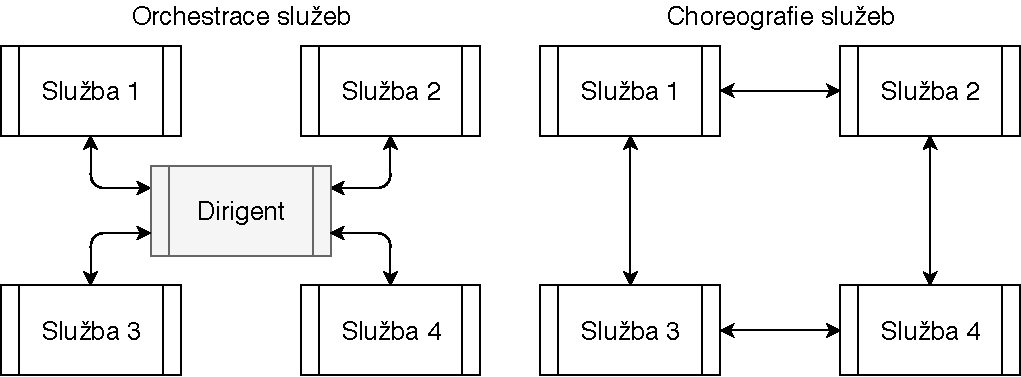
\includegraphics[keepaspectratio=true, width=0.8\linewidth]{figures/choreography-orchestration.pdf}
    \caption{Porovnán\'{\i} orchestrace a choreografie služeb~\cite{cerny2017disambiguation}}
    \label{fig:choreography-orchestration}
\end{figure}

\section{Nedostatky současného př\'{\i}stupu}\label{sec:shortcomings}

\goal{Navázán\'{\i} na předchoz\'{\i} sekci}
Jak jsme zjistili v předchoz\'{\i}ch odstavc\'{\i}ch, \gls{SOA} se zaměřuje zejména na
dělen\'{\i} systému na služby a detailně rozeb\'{\i}rá formu jejich vzájemné komunikace.
Neodpov\'{\i}dá ale na několik závažn\'ych otázek, se kter\'ymi se v praxi musej\'{\i}
architekti informačn\'{\i}ch systémů vypořádat, aby architektura byla schopná uspokojivě
plnit požadavky, které jsou na n\'{\i} kladené.

\goal{Problémy SOA a průřezov\'ych problémů}
Jelikož jedn\'{\i}m z c\'{\i}lů \gls{SOA}, potažmo microservices, je co nejv\'{\i}ce izolovat
jednotlivé služby, maj\'{\i} tyto architektury tendenci duplikovat části kódu
zajišťuj\'{\i}c\'{\i} funkcionalitu, která vyžaduje konzistentn\'{\i} zpracován\'{\i} ve v\'{\i}ce
službách~\cite{cerny2017disambiguation}, tzv. \textit{průřezov\'ych
problémů} (z anglického \textit{cross-cutting concerns}).
Př\'{\i}kladem mohou b\'yt právě byznysová pravidla~\cite{cemus2014aspect}, která je potřeba
zohlednit v rámci různ\'ych byznysov\'ych kontextů realizovan\'ych ve v\'{\i}ce službách.
Mezi dalš\'{\i} př\'{\i}klady se řad\'{\i} logován\'{\i}, monitoring či sběr dat
o telemetrii procesů.

\goal{Nast\'{\i}něn\'{\i} konkrétn\'{\i}ho př\'{\i}kladu}
Abychom si mohli lépe představit diskutovan\'y problém, znázorněmě
si ho na konkrétn\'{\i}m př\'{\i}kladu. Uvažme e-commerce systém
skládaj\'{\i}c\'{\i} se z několika služeb naprogramovan\'ych v různ\'ych technologi\'{\i}ch,
organizovan\'ych kolem jeho byznysov\'ych funkc\'{\i}.
Jedna služba obsluhuje byznysové operace vázaj\'{\i}c\'{\i}
se na uživatele systému, jejich registraci a administraci. Druhá
služba realizuje operace s produkty, jejich vytvářen\'{\i}, úpravu,
správu skladov\'ych zásob a informace o dostupnosti. Třet\'{\i} služba je
zodpovědná za vytvářen\'{\i} a správu objednávek, informován\'{\i} uživatelů
o změnách jejich stavů a vytvářen\'{\i} statistik a reportů pro management.
Čtvrtá služba má na starosti účetnictv\'{\i}, tedy vystavován\'{\i} a přij\'{\i}mán\'{\i}
faktur a komunikaci s bankovn\'{\i}mi službami o potvrzen\'{\i} přijat\'ych plateb.
Posledn\'{\i}, pátá služba, poskytuje uživatelské a umožňuje komfortn\'{\i} obsluhu systému.

\goal{Konkrétn\'{\i} problémy zpracován\'{\i} průřezov\'ych problémů na př\'{\i}kladu}
Jak již v\'{\i}me, každá byznysová operace má své preconditions, které musej\'{\i} b\'yt splněny,
aby mohla b\'yt vykonána. Operace má také post-conditions, které musej\'{\i} b\'yt
aplikovány po skončen\'{\i} operace. Např\'{\i}klad při vytvářen\'{\i} faktury za
objednávku mus\'{\i} b\'yt zvalidována fakturačn\'{\i} adresa, bez n\'{\i}ž nemůže
b\'yt faktura vystavena. Pokud chceme ušetřit práci účetn\'{\i}kům, kteř\'{\i} by
v př\'{\i}padě nevalidn\'{\i} adresy musely kontaktovat zákazn\'{\i}ka – pokud vůbec
takovou možnost maj\'{\i} – mus\'{\i}me tento fakt zohlednit již při vytvářen\'{\i} objednávky.
Proces vytvářen\'{\i} objednávky ale realizuje jiná služba, než vystavován\'{\i} faktur.
V ideáln\'{\i}m př\'{\i}padě bychom chtěli zákazn\'{\i}ka upozornit na nevalidn\'{\i} fakturačn\'{\i}
adresu dynamicky ještě před odeslán\'{\i}m objednávkového formuláře př\'{\i}mo v uživatelském
rozhran\'{\i}~\cite{cemus2017separation}. Pro lepš\'{\i} představu je problém znázorněn na
obrázku~\ref{fig:service-cutting},

\goal{Náročná údržba a reakce na změnu požadavku}
Z tohoto př\'{\i}kladu je jasně vidět, že stejná funkcionalita se prom\'{\i}tá
do tř\'{\i} služeb, z nichž každá má zodpovědnost za jiné byznysové operace.
To znamená, že stejn\'y kód, kter\'y realizuje validaci fakturačn\'{\i} adresy,
mus\'{\i} b\'yt implementován v každé ze služeb – v našem př\'{\i}padě nav\'{\i}c ve třech
různ\'ych programovac\'{\i}ch jazyc\'{\i}ch. Ve chv\'{\i}li, kdy vzejde požadavek na změnu
validace fakturačn\'{\i} adresy \textendash řekněme, že chceme zobecnit
validaci PSČ a umožn\'{\i}me přij\'{\i}mat i jeho tvar s mezerou – mus\'{\i}me stejnou změnu
provést konzistentně na třech různ\'ych m\'{\i}stech, všechny tři služby znovu
sestavit a nasadit ve správném pořad\'{\i} tak, aby nedošlo ke stavu,
kdy jedna služba přijme nov\'y tvar PSČ, ale navazuj\'{\i}c\'{\i} služba ho nen\'{\i}
schopna zpracovat.

\goal{Microservices neř\'{\i}ká nic o tom, jak velké je mikro}
Pozorn\'y čtenář může nam\'{\i}tnout, že problém validace fakturačn\'{\i}ch adres by
bylo možné vyřešit vyčleněn\'{\i}m této funkcionality
do samostatné služby a vystavit jej\'{\i} rozhran\'{\i} pro ostatn\'{\i} služby,
v souladu s nosnou myšlenkou microservices. Je pravda, že microservices
v názvu nese slovo \uv{micro} a evokuje tak, že služby by měly b\'yt co nejmenš\'{\i}
a nést co nejméně zodpovědnosti. Může ale nastat stav, kdy je služba př\'{\i}liš malá?
Pokud služby ponesou př\'{\i}liš málo odpovědnosti,
přináš\'{\i} to s sebou několik problémů, které je nutné zvážit. Mus\'{\i}me m\'{\i}t na paměti, že
nasazen\'{\i} a provoz každé služby s sebou přináš\'{\i} náklady nav\'{\i}c
a zvyšuje časové nároky na jejich v\'yvojáře a administrátory.
Komunikace služeb po s\'{\i}ti je nav\'{\i}c podstatně pomalejš\'{\i} a náchylnějš\'{\i} na
chybu, než komunikace jednotliv\'ych komponent v rámci jednoho procesu.
S rostouc\'{\i}m počtem \textit{průřezov\'ych problémů} by tak i rychle rostl
počet služeb v systému a celkové náklady na jeho v\'yvoj a údržbu.

\begin{figure}
    \centering
    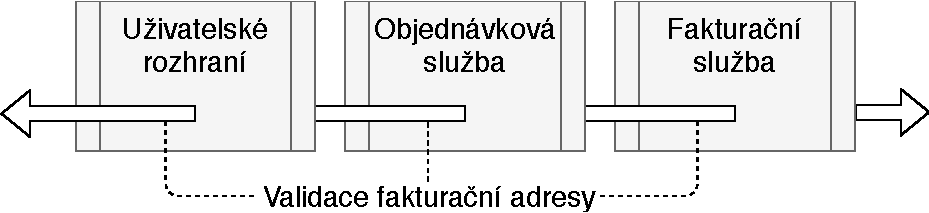
\includegraphics[keepaspectratio=true, width=0.8\linewidth]{figures/service-cutting.pdf}
    \caption{Př\'{\i}klad zásahu jedné funkcionality do v\'{\i}ce služeb}
    \label{fig:service-cutting}
\end{figure}

\goal{Shrnut\'{\i} problémů}
Na př\'{\i}kladu můžeme vidět, že existuje typ problémů, které v rámci architektury
orientované na služby při využit\'{\i} současného př\'{\i}stupu nejsme schopni uspokojivě
vyřešit na jednom m\'{\i}stě a vedou k duplikaci znalost\'{\i} na v\'{\i}ce m\'{\i}stech systému.
Taková duplikace může vést k zv\'yšenému riziku lidské chyby v\'yvojáře a t\'{\i}m k
nekonzistentn\'{\i}mu chován\'{\i} systému. Nav\'{\i}c zvyšuje cenu na v\'yvoj a údržbu systému.

\section{Identifikace požadavků na implementaci frameworku}\label{sec:implementation-requirements}

Z př\'{\i}kladu popsaného v\'yše můžeme identifikovat požadavky, které by měly
b\'yt zohledněny při návrhu a implementaci frameworku, kter\'y bude sloužit
pro centráln\'{\i} administraci a automatickou distribuci byznysov\'ych pravidel
v architektuře orientované na služby.

Framework, resp. jeho knihovny, by měly umožňovat:

\begin{itemize}
    \item{Definice byznys kontextů pomoc\'{\i} platformně nezávislého doménově specifického jazyka srozumitelného pro doménové experty}
    \item{Zápis preconditions a post-conditions pravidla jednotliv\'ych byznys kontextů}
    \item{Možnost jednoho kontextu rozšiřovat jiné kontexty}
    \item{Možnost centrálně spravovat byznysové kontexty, včetně úpravy stávaj\'{\i}c\'{\i}ch a vytvářen\'{\i} nov\'ych kontextů, to vše dynamicky za běhu systému}
    \item{Automatickou distribuci kontextů, vyhodnocován\'{\i} jejich preconditions a aplikaci post-conditions}
    \item{Možnost využ\'{\i}vat framework na v\'{\i}ce plaformách}
\end{itemize}

\section{Shrnut\'{\i}}

V této kapitole jsme nast\'{\i}nili problematiku vysoké komplexity modern\'{\i}ch informačn\'{\i}ch systémů
a z toho vypl\'yvaj\'{\i}c\'{\i} požadavky na jejich architekturu. Analyzovali jsme koncept byznysov\'ych
pravidel a byznysov\'ych kontextů. Dále jsme prozkoumali architekturu orientovanou na služby, jej\'{\i}
v\'yhody a nev\'yhody, jej\'{\i} modern\'{\i} evoluci v podobě microservices a identifikovali jsme nedostatky
současn\'ych př\'{\i}stupů v řešen\'{\i} průřezov\'ych problémů, které zasahuj\'{\i} do v\'{\i}ce služeb najednou. Nakonec
jsme vyjmenovali požadavky, které by měl splňovat framework, jež bude v\'ystupem této práce.
